\documentclass[%
 aapm,
 mph,%
 amsmath,amssymb,
%preprint,%
 reprint,%
%author-year,%
%author-numerical,%
]{revtex4-2}

\usepackage{titlesec}
% Format section headings with sans-serif font
\titleformat{\section}
{\large\bfseries\sffamily}
{\thesection}{1em}{}
% Format subsection headings with sans-serif font
\titleformat{\subsection}
{\bfseries\sffamily}
{\thesubsection}{1em}{}

% Format subsubsection headings with sans-serif font
\titleformat{\subsubsection}
{\bfseries\sffamily}
{\thesubsubsection}{1em}{}
\usepackage{graphicx}% Include figure files
\usepackage{xcolor}
\usepackage{breqn}
\usepackage{hyperref}
\hypersetup{
    colorlinks = true,
    linkcolor={red!50!black},
    citecolor={blue!50!black},
    urlcolor={blue!80!black}
}
\begin{document}


\title[PHY401 TermPaper: Spring Semester 2022]{Clocks as Measurement Devices, but do we really measure time?}
%\thanks{Footnote to title of article.}

\author{Aditya Dev (MS19022), Jai Samarth (MS19092), Pratiyush Vashisht (MS19073)}
\affiliation{\text{Department of Physics} \\
Indian Institute of Science Education and Research Mohali}%


\date{\today}% It is always \today, today,
             %  but any date may be explicitly specified

\begin{abstract}
We presents a physical construct of a Cesium Standard type of atomic clock which were the first kind to replace the ``ephemeris second". This paper also discusses non-periodic clocks based on irreversible phenomenon. 
\end{abstract}

\maketitle
\tableofcontents

\vspace{10pt}

\section{Physical Construction of the Cesium Standard}

\begin{figure}[ht]
    \centering
    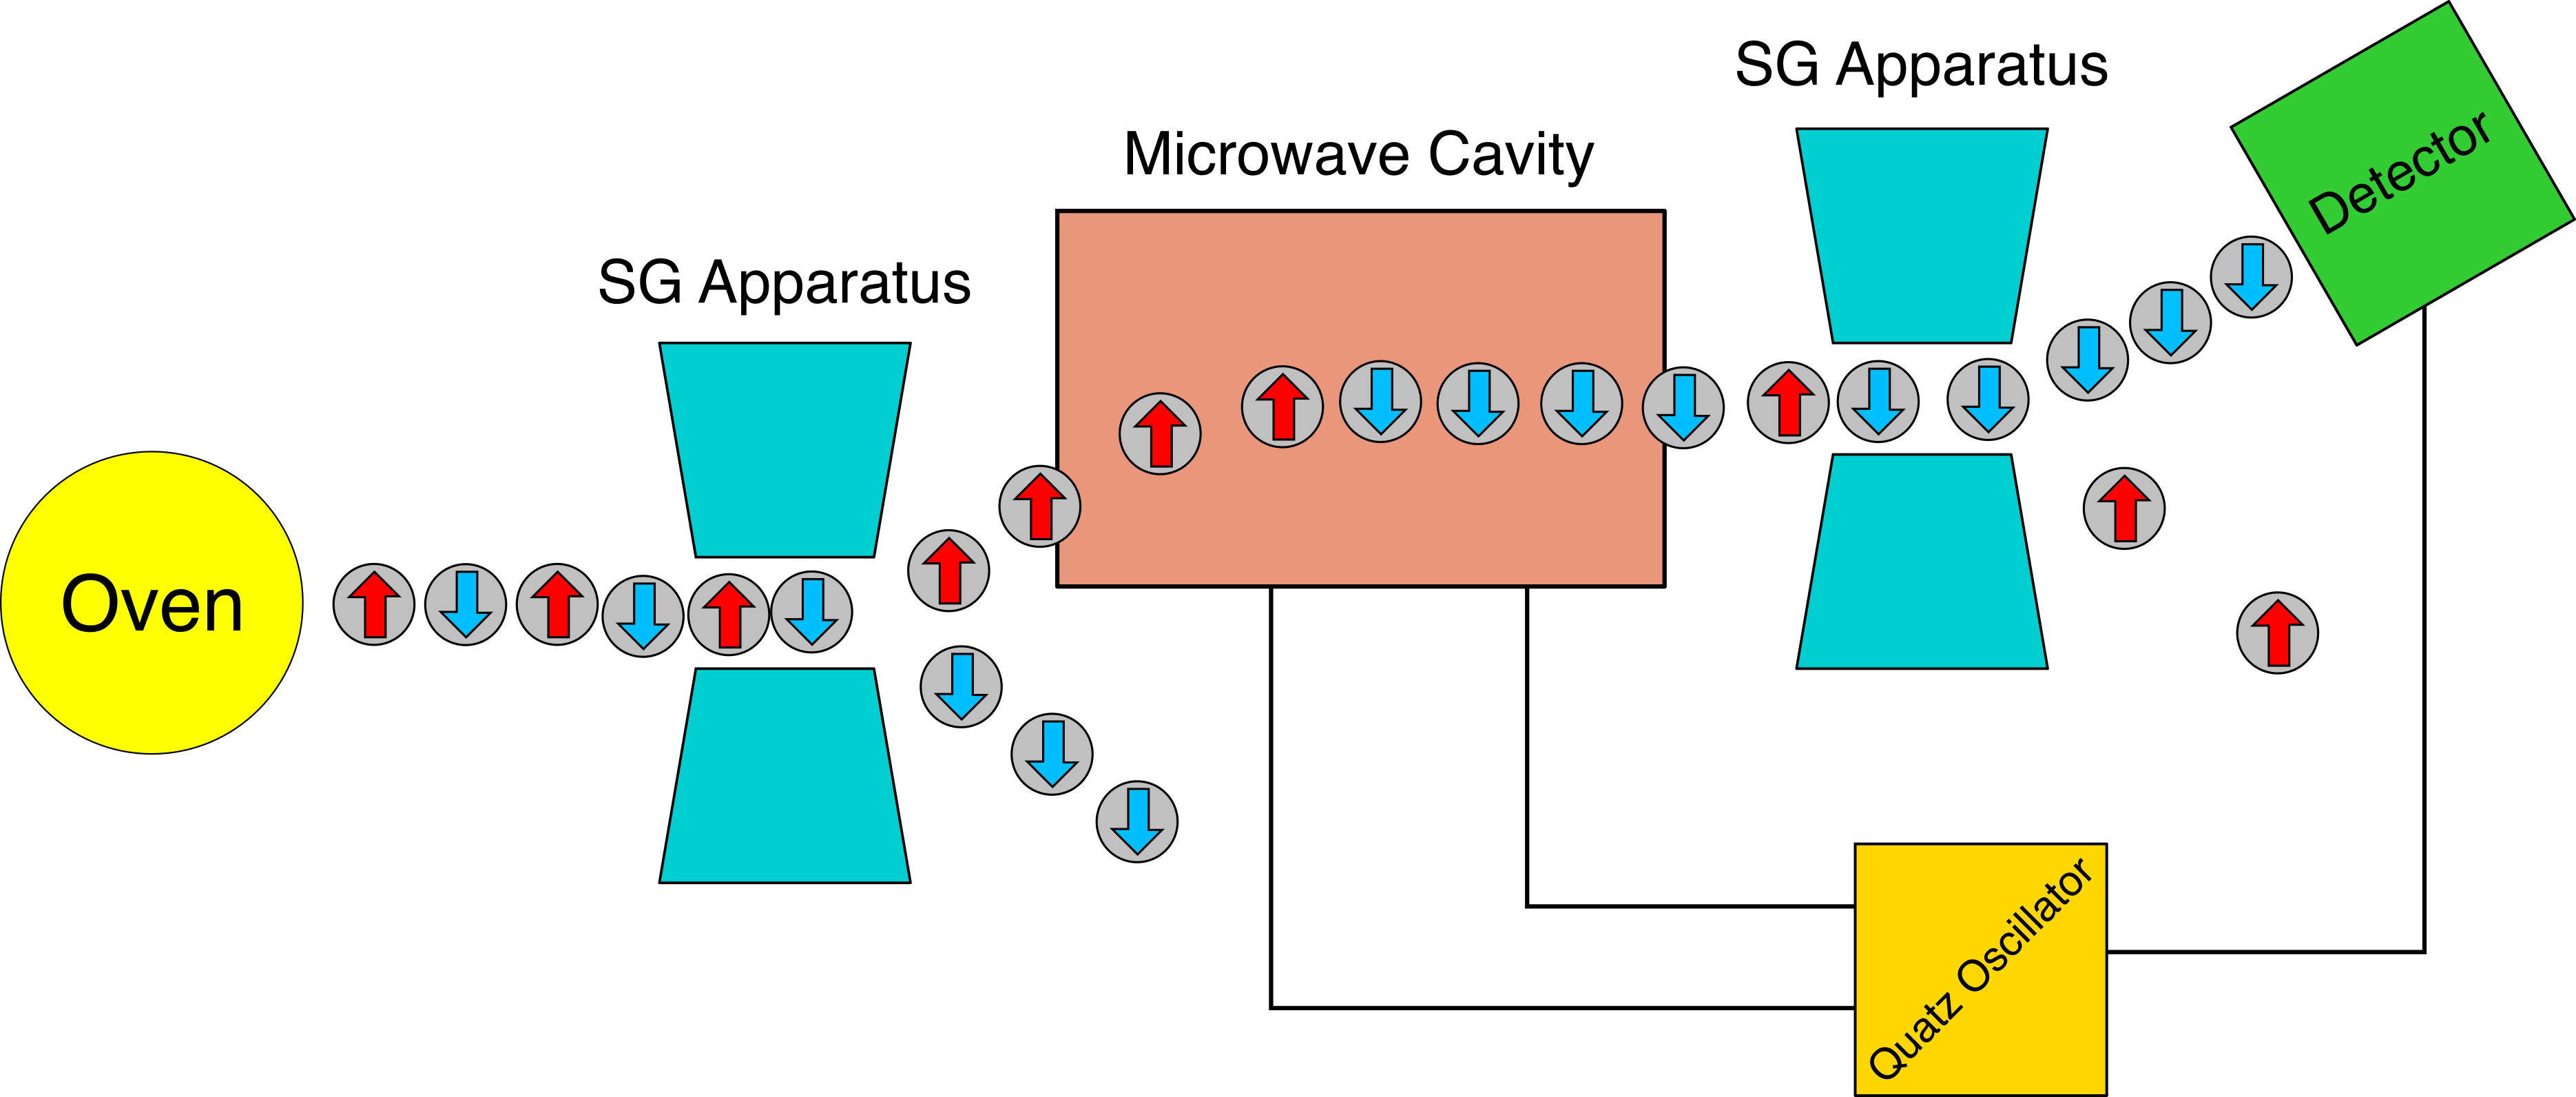
\includegraphics[width =0.48\textwidth]{rect1076.png}
    \caption{Simplified Schematic}
\end{figure}

In this section we'll primarily go through the physical construct of a Cesium Standard type of atomic clock which were the first kind to replace the ``ephemeris second".
The entire space traversed by the Cesium atoms is maintained under high vacuum. Cesium atoms originate from an oven maintained at over
$100^\circ$ C and pass through a collimator that creates a narrow beam of atoms. This beam makes its way to a Stern-Gerlach apparatus where 
the atoms are subjected to a magnetic field with steep transverse gradient and separated into the two states (F = 4 and 
F = 3) respectively. One of the beams is sent to a microwave cavity oscillating at a frequency close to the hyperfine transition energy (9,192,631,770 Hz).
Now, when the microwave frequency is equal to this frequency, resonance is achieved, and the state of the beam is flipped.
The closer the frequencies are, the larger fraction of the beam is flipped. After this, another Stern-Gerlach apparatus selects the flipped beam and then
passes it into a detector. This detector consists of a hot-wire ionizer that ionizes the Cesium atoms and a mass spectrometer which 
selects the previously ionized Cesium atoms. Finally, the ionized cesium atoms hit a photomultiplier tube plate and generate an electrical signal.

\begin{figure}
    \centering
    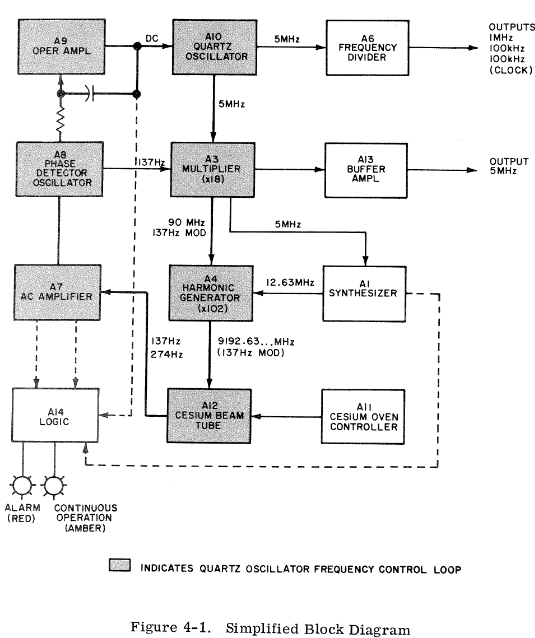
\includegraphics[width = 0.4\textwidth]{device.png}
    \caption{Schematic \cite{hpclock}}
\end{figure}

Now, the closer our microwave frequency is to the hyperfine transition energy, the larger will be the generated signal. To get as close to this
frequency as possible we first generate a signal using a quartz oscillator at 5 MHz. This signal was multiplied 18 times to get
a 90 MHz signal. This signal is passed into a harmonic generator which generates a 9180 MHz signal (102th harmonic) from this 90 MHz signal. This signal
is then later mixed with a digital PLL synthesized 12.631770 MHz signal, finally giving a 9192631770 Hz signal. This signal is now modulated with
a 137 Hz signal, and a PLL can now lock on the hyperfine transition frequency. The PLL will generate twice the modulated frequency if the modulated signal carrier wave (9192631770 Hz) is exactly the same as the cesium hyperfine transition frequency. In case of any deviation, the output will include the 137 Hz modulation which was
absent in the locked state of the PLL. The information featured here can be found in \cite{hpclock} \& \cite{major2013quantum}.



\subsection{Physics behind the cesium clock }
The Cesium clock uses the transition between the spin states of the cesium nucleus, which are the hyperfine structures, and produces a frequency that is so regular that is is used to define time. Hyperfine structures \cite{encyclbritannica} are defined by small shifts in the degenerate energy levels and the resulting splitting in those energy levels due to \textbf{electromagnetic multipole interaction} between the nucleus and the electron cloud. Similar to an electron we have nuclear spin. The interaction of nucleus spin with the internal magnetic field, the magnetic field produced by the electron cloud, is the cause of splitting in the spectral lines. The spectral lines are observed using interferometry. 

These effects are very small and each splitting is associated with a quantum level, denoted by F. Although the spin angular momentum of a nucleus is of the order similar to the electron. But its magnetic moment, which governs the energy of the atomic levels, is relatively small. 


 Cesium contains \emph{(Z=55)} protons and \emph{(N=78)} neutrons. Clearly its an odd-even nuclei. The shell model \cite{povh2012particles} of Cesium nuclei has all the neutrons to be paired up and does not contribute to the spin of nucleus, and hence they do not interact with the magnetic field. The proton whereas odd in number, do contribute to the total spin of the nucleus. The last 5 protons lies in the 1g$_{7/2}$ out of which 2 protons are paired and there is one unpaired proton. The last proton in 1g$_{7/2}$ has total angular momentum $I_{nucl}  = 7/2$ corresponding to the ground state of nucleus. We define hyperfine splitting as \textbf{F}= 
 $I_{nucleus} + J_{electron}$. The total angular momentum of valence electron is given by \emph{J$_{ele}$=L+S}. For the electron we have L=0 corresponding to the orbital S of the cesium valence electron. The Spin value can be $S = \frac{+}{} \frac{1}{2}$. Therefore, the total angular momentum coupling is given by:
\begin{equation}
    |I + J| \le F \le |I- J| 
\end{equation}
\begin{equation}
    F =  \frac{7}{2} \pm \frac{1}{2}
\end{equation}
We have values of \emph{F = 4,3} corresponding to spin, S=+$\frac{1}{2}$ , S= -$\frac{1}{2}$. Thus, we have the transition corresponding to F=4 to F=3 which are extremely precise to work as a clock. The energy gap corresponding to the two F values is given $\Delta$E = h$\nu_0$. Here $\nu_0$ is the frequency of electromagnetic radiation ,which when applied to cesium gives the exact transition between the two states. 

\subsection{Hamiltonian Of Atomic Clock}
The Hamiltonian of the system(Atomic clock) \cite{wikipedia:1108487361} depends on the nuclear multipole moments interacting with internally generated fields, due to the electron cloud. For hyperfine structures we have the dominant term in the hamiltonian is the magnetic dipole moment given by:
\begin{equation}
    \mu_I = g_I\mu_NI
\end{equation}
We have the \textbf{Hamiltonian} of the form.

\begin{equation}
\hat{H} = -\vec{\mu_I}\cdot \Vec{B} 
\end{equation}

Here, $\vec{B}$ is the magnetic field due to electron cloud($\vec{B_{el}}$)
\begin{center}
$\vec{B_{el}} = \vec{B^l_{el}} +\vec{B^s_{el}}$ 
\end{center}
The magnetic field at the nucleus due to the motion of a single electron at a distance \emph{r} from the nucleus is given by:
\begin{equation}
    \vec{B^l_{el}} = \frac{\mu_0}{4\pi} \Big( \frac{-ev\times(-r)}{r^3}\Big)
\end{equation}
\begin{equation}
    \vec{B^l_{el}} = -2\mu_B \frac{\mu_0}{4\pi} \frac{1}{r^3}\Big( \frac{r\times(M_ev)}{\hbar}\Big)
\end{equation}
here, $\vec{\mu_B}$ = $\big(\frac{e\hbar}{2M_e}\big)$. on adding the spin magnetic moment $\mu_s$ we get the final form of the magnetic field of a dipole moment,as \cite{Jackson:100964} :
\begin{equation}
    \vec{B^l} = \frac{\mu_0}{4\pi r^3}\Big(3(\mu_s \cdot \hat{r})\hat{r}-\mu_s \Big) +\frac{2\mu_0}{3}\delta^3(r)
\end{equation}
 The complete magnetic dipole contribution to the hyperfine Hamiltonian \cite{Soliverez_1980} is given as:\\
\begin{equation}
\begin{aligned}
\hat{H_D} = 2g_I\mu_N\mu_B\frac{\mu_0}{4\pi}\frac{1}{L_z}\sum\frac{\hat{l}_{zi}}{r^3_i}I\cdot L\\ + g_I\mu_N g_s\mu_B \frac{\mu_0}{4\pi} \frac{1}{S_z} \sum \frac{\hat{s}_{zi}} {r^3_i} {3(I\cdot \hat{r})(S \cdot \hat{r}) - I\cdot S} \\ + \frac{2}{3}g_I\mu_N g_s\mu_B\mu_0 \frac{1}{S_z}\sum \hat{s}_{zi}\delta^3(r_i)I\cdot S
\end{aligned}
\end{equation}
\emph{1.} The $1^{st}$ term correspond to the energy of the nuclear dipole in the field due to electronic orbital angular momenta. \emph{2.} The term $2^{nd}$ corresponds to the "finite distance" interaction of the nuclear dipole due to $e^-$ spin magnetic moment.\\
\emph{3.} The $3^{rd}$ term corresponds to the "Fermi Contact" (interaction of nuclear dipole with spin dipoles.It is only non-zero for states with a finite electron spin density at the position of nucleus. 

The Hamiltonian For the hyperfine structure is given as \cite{steck2003cesium}:

%\begin{aligned}
\begin{dmath}
H_{hfs} = A_{hfs} I \cdot J + B_{hfs} \times \left( \frac{(3(I\cdot J)^2+\frac{3}{2}I\cdot J - I(I+1)J(J+1)} {2I(2I-1)j(2J-1)}\right)
\end{dmath}

%\end{aligned}
This hamiltonian leads to the hyperfine energy shift of 
\begin{dmath}
    \Delta E_{hfs} = \frac{1}{2}A_{hfs}K+ B_{hfs}  \times \left(\frac{ \frac{3}{2}K(K+1) -2I(I+1)J(J+1)}{2I(2I-1)2J(2J-1)}\right)
\end{dmath}
Here $K = F(F+1)-I(I+1)-J(J+1)$, $A_{hfs}$ is the magnetic dipole constant. $B_{hfs}$ is the electric quadropole constant corresponding to the nuclei having spin $I\ge 1$.

%\vspace{0.5cm}
\paragraph{Interaction Hamiltonian}
Each of the hyperfine(F) energy levels contains 2F+1 magnetic sublevels that determine the angular distribution of the electron wave function. These sublevels are degenerate in the absence of external electric field. As we apply the external magnetic field the degeneracy is broken and the sub levels splits. The Hamiltonian describing the atomic interaction with the magnetic field.\\
\begin{equation}
\begin{aligned}
    H_B = \frac{\mu _B}{\hbar}(g_SS + g_LL + g_II)\cdot B\\
        = \frac{\mu_B}{\hbar}(g_SS_Z + g_LL_Z + g_II_z) B_Z
\end{aligned}
\end{equation}
If the energy shift due to the magnetic field is small compared to the fine-structure constant splitting, then J=L+S is a good quantum number,the $H_{inter}$ become \\

\begin{equation}
\begin{aligned}
    H_B = \frac{\mu_B}{\hbar}(g_JJ_Z + g_II_Z) B_Z
\end{aligned}
\end{equation}
 
 For weak magnetic field, the interaction hamiltonian\cite{steck2003cesium} $H_B$ perturbs the zero-field eigenstates of $H_{hfs}$.To lower order, levels split linearly as shown in the equation.This spliting is called the Zeeman Effect.
\begin{equation}
\Delta E_{|F,m_F>} = \mu_B g_Fm_FB_Z    
\end{equation}
For strong fields the interaction term dominates the hyperfine energies, so that the hyperfine Hamiltonian perturbs the strong-field eigenstates $\left|J,m_J, I,m_I\right\rangle$.\\
The Briet-Rabi formula is useful in finding the small-field shift of the "clock-transition" between the \emph{$m_F$=0} sublevels of the two hyperfine ground states.Using \emph{$m=m_F$} for small magnetic fields,the frequency of the clock is,
\begin{equation}
\Delta w_{clock} = \frac{(g_J-g_L)^2\mu^2}{2\hbar \Delta E_{hfs}}B^2
\end{equation}

\subsection{Why we choose Cesium}
We choose Cesium as our element for the atomic clock construction. Since hyperfine structures are only formed for the element having non even-even nuclei. Because for even-even nuclei, total nuclear spin equals to zero. Thus the nucleus do not interact with magnetic field and we just get the fine structures. For Cesium we have even-odd nuclei,implies one unpaired nucleon. The size of the atom is large thus the velocity of atom in vacuum is slower which helps in better splitting of the atoms in the magnetic field. Therefore we get a much better distribution of particle with different spin orientation.\\
The only valence electron of Cesium lies in the \textbf{S}-orbital (ground state) with corresponding (l=0) and (S=+-$\frac{1}{2}$) provides two very well,precise values of F=3,4. This gives a unique transition levels,where as if we have other than (l=0) there are more than two quantum levels of F, thus will have different transition levels which are not good for the construction of clock.

\section{Non Periodic Clocks?}
A clock is often presented as the epitome of a reversible and predictable dynamical system. But like any other physical device, a clock is also subject to the laws of thermodynamics. 
Irreversible clocks have long been used, water clocks for example, and a particular irreversible clock is in common usage; Radiocarbon dating is based on the stochastic and irreversible decay of a radionuclide - $C^{14}$

\textbf{Radoiocarbon Dating:} The probability of a single radionuclide not to decay in a time t is $\exp(-\gamma t)$, where $\gamma$ is called the decay rate. Given an ensemble of undecayed radionuclides, the number that have decayed after some time $t$
is a Poisson distributed stochastic variable $N$ with mean
$\gamma t$. Thus, given a count of the number of radionuclides
that have decayed, $N$, we may estimate the time that has
elapsed as
\begin{equation}
    t_{est} = \frac{N}{\gamma}
\end{equation}

The error in this estimate is given by the fluctuations in
the final count $\delta N$ for a fixed estimate test. . Since for a Poisson process the variance is equal to the mean, one
finds the relative error is:
\begin{equation}
    \frac{\delta t_{est}}{t_{est}} = \frac{1}{\sqrt{\gamma t_{est}}}
\end{equation}
\textbf{Mach's Thermodynamic Clock}
Mach introduced a temperature clock in an attempt to ground an understanding of time in our sense perception of irreversible processes. Mach’s clock is a thermodynamic system in which three identical materials, initially held at different temperatures, are placed in thermal contact but thermally isolated from the rest of the universe. 
Being an adiabatic system, the total energy of system will be conserved: 
\begin{equation}
    \dot{U} = s\left(\dot{T_1} +\dot{T_2} +\dot{T_3} \right)
\end{equation}
where $c$ is the specific heat. The above equation gives, \(
T_1(t) + T_2(t) + T_3(t) = T_1(0) + T_2(0) + T_3(0)
\)
Newton's law of cooling gives for this case: 
\begin{equation}
    \dot{T_1} = k(T_3 - T_1) + k (T_2- T_1)
\end{equation}
$k$ is constant with dimensions of inverse time. Using same relations for other temperatures.
\begin{equation}\label{eq:Ttilde}
    \Tilde{T} = T_1 (\tau)  = A \exp ^{-3 k \tau}
\end{equation}
where $A =  \Tilde{T} - T_1(0)$ is a constant and we have defined
the initial average temperature as  $\Tilde{T} = (T_1(0) + T_2(0) +T3(0))/3$. This is very like radioactive decay. Equation \ref{eq:Ttilde} implies

\begin{equation}
\frac{\Delta T_1}{T_1} + \frac{\Delta \tau}{\tau _{est}} = 0
\end{equation}
where we have defined an estimated time by $\tau _{est} = 1/{3k}$ in
analogy with radioactive decay. \cite{optomechanicalclock}

\subsection{Internal and External Time}

[This  section is taken from \cite{borghi2012clock}]

In physics the concept of time is used in 2 different ways:
\begin{itemize}
    \item As an external attribute of motion.
    \item As an implicit variable that measure the internal evolution of a system.
\end{itemize}
The first one is explicitly used in mechanics and the second, implicitly in thermodynamics.  The mechanical evolution is related to the change in the position of a body with respect to others, the thermodynamic evolution of a system is linked to processes that involve it internally and might not have relationships with the environment, thus with the external space of relations. In the first case time is like a label attached to the system, in the second it is
a quantity that informs us of its intrinsic evolution.

\paragraph{Atomic clocks} are influenced by the distribution of matter and energy in which they are immersed. These tools reduce the measure of time to a counting of ideally reversible periodic oscillations. As a measuring instrument of irreversible time we can use a radioactive clock, which quantifies the increasing product of decay and allows us to measure the increase in the amount of change and transformation that occurs in the system (if isolated) to which it belongs. We know that radioactive decay is an irreversible process, consisting in the production of a daughter from a parent substance.
Let us consider the law:
\begin{equation}\label{eq:decay}
    N = N_0 \left( 1 - e^{- \frac{t}{\tau}}\right)
\end{equation}

where $N$ expresses the quantity of the substance produced by the decay
as a strictly increasing function of time t. We observe that the value
of N can be considered a direct measure of thermodynamic time: it
quantifies, in units of $N_0$, the duration of the decay. If we solve equation \ref{eq:decay}, we can calculate the corresponding value of t: the quantification of
$t$ is not necessary, it is simply useful.
\begin{equation}\label{eq:deacytime}
    t = \tau \ln \left( \frac{N_0}{N_0 - N}\right)
\end{equation}
We can convert $t$ in seconds (it's in units of $\tau$) using the known value of the average lifetime of the substance. This procedure has an important physical and conceptual meaning: it makes us understand that this clock measures internal proper time using a non periodic and irreversible phenomenon. By varying the radioactive substance (the dynamic heart of the instrument) we get another clock with a different $\tau$ , which
determines the rate of decay. The incommensurability of the measures
of durations obtained by different radioactive clocks prevents us from
concluding that they can be used to measure absolute time. Nor can we
conclude that radioactive clocks can be relativistic clocks, as they are
inadequate for quantifying the effects expected from Einstein’s theory.

Equation \ref{eq:decay} implicitly says that a
population of $N_0$ atoms decays into a daughter substance, producing a
measurable amount of decay. The quantification of this product is the
experimental consequence of the increase of entropy: the progressive increase of $N$ is a proof. It could be argued that a radioactive clock is not necessarily an isolated system: the principle of increasing entropy applies to isolated systems or more generally to systems and environments, therefore to the whole universe as an isolated system. However, if we experimentally test that it is not influenced on the fields in which it is immersed nor on acceleration, we can conclude that this clock forms an isolated system and then it measures internal proper time. In agreement with the working hypotheses, every theoretical
formalization implies a conceptual framework within which the operational definition of physical time is given, thus it is necessary to clearly distinguish the specific areas of investigation of the different theories. Thermodynamic time, measured by clocks inside of which periodic phenomena are not produced, but energy transformations associated with irreversible processes, quantifies the real degradation of matter and energy. The irreducibility of thermodynamic time to absolute or relativistic time implies that in any specific area specific clocks should be designed.

\textbf{Two not identically constructed clocks quantify different physical processes and furnish different measurements. So the results of experiments on the measure of time intervals do not express the properties of time itself, but of the objects or phenomena that these instruments are called upon to investigate.}

\bibliography{aapmsamp}% Produces the bibliography via BibTeX.

\end{document}
%
% ****** End of file aapmsamp.tex ******
